% Compile with XeLaTeX, TeXLive 2013 or more recent
\documentclass{beamer}

% Base packages
\usepackage{fontspec}
\usepackage{xunicode}
\usepackage{xltxtra}

\usepackage{amsfonts}
\usepackage{amsmath}
\usepackage{longtable}
\usepackage{csquotes}
\usepackage{standalone}

% Setup fonts
\newfontfamily\russianfont{CMU Serif}
\setromanfont{CMU Serif}
\setsansfont{CMU Sans Serif}
\setmonofont{CMU Typewriter Text}

% Setup Russian hyphenation. NOTE: this declaration *must* come after fontspec's font declarations,
% or a mysterious (but harmless in other respects) error "Improper `at' size (0.0pt), replaced by 10pt." would appear.
\usepackage{polyglossia}
\defaultfontfeatures{Scale=MatchLowercase, Mapping=tex-text}

\setdefaultlanguage[spelling=modern]{russian} % for polyglossia
\setotherlanguage{english} % for polyglossia

% Vector drawings 
\usepackage{tikz}
\usetikzlibrary{shapes, calc, arrows, fit, positioning, decorations, patterns, decorations.pathreplacing, chains, snakes}
\usepackage[siunitx]{circuitikz}

% Be able to insert hyperlinks
\usepackage{hyperref}
\hypersetup{colorlinks=true, linkcolor=black, filecolor=black, citecolor=black, urlcolor=blue , pdfauthor=Grigory Rechistov <grigory.rechistov@phystech.edu>, pdftitle=Моделирование OpenRISC 1000 на Wind River Simics}
% \usepackage{url}

% Misc optional packages
\usepackage{underscore}
\usepackage{amsthm}

% A new command to mark not done places
\newcommand{\todo}[1][Напиши меня]{{\color{red}TODO\ #1}}


\title{Компьютерная симуляция }
% \subtitle{Курс «Программное моделирование вычислительных систем»}
\subject{Лекция}
\author[Григорий Речистов]{Григорий Речистов \\ \small{\href{mailto:grigory.rechistov@intel.com}{grigory.rechistov@intel.com}}}
\date{\today}
\pgfdeclareimage[height=0.5cm]{intel-logo}{../images/intel.png}
\logo{\pgfuseimage{intel-logo}}


\typeout{Copyright 2014 Grigory Rechistov}

\usetheme{Berlin}
\setbeamertemplate{navigation symbols}{}%remove navigation symbols

\begin{document}

\begin{frame}
\titlepage
\end{frame}

\begin{frame}
\tableofcontents
\end{frame} 

\begin{frame}{Обо мне}

\raggedleft 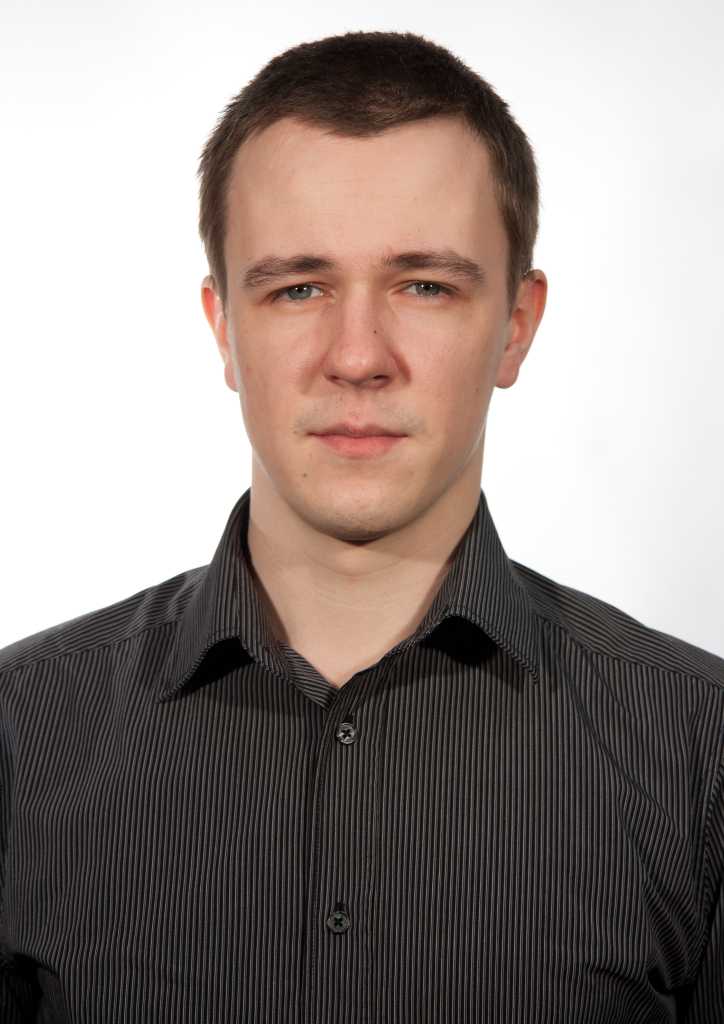
\includegraphics[height=0.3\textheight]{./grigory-rechistov}

\begin{itemize}
\item Закончил МФТИ в 2010 г.
\item Защитил диссертацию к.т.н в 2013 г.
\item Работаю в Московском отделении Intel 
\item Интересы: симуляция, образование, спорт

\end{itemize}


\end{frame} 

\begin{frame}{Почему симуляция актуальна для \emph{вас}?}

\begin{enumerate}
\item Это интересно --- как работают компьютеры внутри!
\item Помогает стать лучшим программистом --- почему код работает именно так, а не иначе (даёт ответы на загадки необъяснимых падений, плохой производительности)
\item Знания востребованы работодателями --- HPC, embedded, gaming, ОС \dots
\item Многие алгоритмы/идеи симуляции являются общими для всей области CS, в т.ч. компиляции, ОС, прикладного ПО.
\end{enumerate}

\end{frame} 

\begin{frame}{Опрос}
Кто из вас знаком с

\begin{enumerate}
\item Архитектурой ЭВМ?
\item Компиляторами?
\item Make
\item Python
\end{enumerate}

\end{frame}

\section{Обзор}

\begin{frame}{Место симуляции в области Computer Science}

\centering

\begin{tikzpicture}[>=latex, font=\small]

\begin{scope}[minimum width = 8cm, node distance = 0.2cm, inner sep=1pt]

\node[draw, ] (schematics) {Схемотехника};
\node[draw, above = of schematics] (digital) {Цифровая электроника};
\node[draw, above = of digital] (rtl-design) {Проектирование микросхем};
\node[draw, above = of rtl-design] (transactions) {Разработка стандартов передачи данных};
\node[draw, above = of transactions] (simulation) {Симуляция};
\node[draw, above = of simulation] (firmware) {Firmware};
\node[draw, above = of firmware] (oses) {Операционные системы};
\node[draw, above = of oses] (drivers) {Драйверы};
\node[draw, above = of drivers] (compilers) {Компиляторы};
\node[draw, above = of compilers] (software) {Прикладные программы};
\node[draw, above = of software] (algorithms) {Алгоритмы};

\end{scope}
\end{tikzpicture}

\end{frame}

\section{Фрактал абстракций цифровой техники}

\begin{frame}{КМОП-транзистор}
\begin{tikzpicture}[>=latex]

\draw[fill=blue!10] (0,0) rectangle (10,-2);
\node at (5,-1.5) {n-подложка (Si)};

\draw[fill=red!10] (0,0) rectangle (4, -1);
\node at (2,-0.5) {p-исток};

\draw[fill=red!10] (6,0) rectangle (10, -1);
\node at (8,-0.5) {p-сток};

\draw[fill=black!10] (3,0) rectangle (7, 0.5);
\node at (5,0.25) {Оксид};

\draw[fill=green!10] (3,0.5) rectangle (7, 1.5);
\node at (5, 1) {Затвор (металл)};

\draw[-o] (1,0) -- (1, 1);
\draw[-o] (9,0) -- (9, 1);
\draw[-o] (5,1.5) -- (5, 2.5);

\end{tikzpicture}
\end{frame}


\begin{frame}{Цифровые вентили}
\begin{circuitikz} 
\draw
(0,0)       node[nigfete, ] (nigfete) {}
(nigfete.D) node[pigfete, anchor=S] (pigfete) {}


(pigfete.G) (nigfete.G) {};


\end{circuitikz} 

\end{frame}

\begin{frame}{Центральный процессор: конвеер}
\begin{tikzpicture}[>=latex]


\end{tikzpicture}

\end{frame}

\begin{frame}{Центральный процессор: минимальная обвязка}
\begin{tikzpicture}[>=latex]

\end{tikzpicture}
\end{frame}

\begin{frame}{Платформа компьютерной системы}
\begin{tikzpicture}[>=latex]

\end{tikzpicture}
\end{frame}

\begin{frame}{Сеть компьютерных систем}
\begin{tikzpicture}[>=latex]

\end{tikzpicture}
\end{frame}



\section{Литература}

\begin{frame}[allowframebreaks]{Литература}
\begin{thebibliography}{99}
    \bibitem{simbook} Основы программного моделирования ЭВМ. Учебное пособие / Г. Речистов, А. Иванов, П. Шишпор, Н. Щелкунов, Д. Гаврилов, В. Пентковский. — Издательство МФТИ, дек. 2012. — ISBN 978-5-7417-0469-1

\end{thebibliography}
\end{frame}


\section{Конец}
% The final "thank you" frame 
\begin{frame}

{\huge{Спасибо за внимание!}\par}

\vfill

Слайды и материалы курса достапны по адресу \url{http://bit.ly/1mr9eCP} % http://atakua.doesntexist.org/wordpress 

\vfill

\tiny{\textit{Замечание}: все торговые марки и логотипы, использованные в данном материале, являются собственностью их владельцев. Представленная точка зрения отражает личное мнение автора. Материалы доступны по лицензии Creative Commons Attribution-ShareAlike (Атрибуция — С сохранением условий) 4.0 весь мир (в т.ч. Россия и др.). Чтобы ознакомиться с экземпляром этой лицензии, посетите \url{http://creativecommons.org/licenses/by-sa/4.0/}}

\end{frame}

% \section{Резерв}

\end{document}


